%----------------------------------------------------------------------------------------
%	CHAPTER 4
%----------------------------------------------------------------------------------------

\chapter{Wyniki badań}
\chaptermark{Wyniki badań} % Tekst, który wyświetli się w nagłówku strony,  jeżeli jest za długi tytuł rozdziałuchapter2.te
Do przeprowadzenia testów aplikacji wykorzystano komputer przenośny Dell Vostro 5515.
Komputer wyposażony został w 32GB pamięci RAM oraz procesor AMD Ryzen 5700u.
Bazowe taktowanie procesora było równe 1.8GHz, natomiast w trybie boost taktowanie rosło do 4.3GHz.
Procesor wyposażono w 8 rdzeni i 16 wątków.
Program testowano na systemie operacyjnym Ubuntu 20.04.5 LTS\@.


\section{Wyniki detekcji tablic rejestracyjnych}
W celu oceny dokładności klasyfikatora służącego do detekcji tablic rejestracyjnych, przygotowano zbiór testowy.
W zbiorze testowym znajdowało się 100 próbek pozytywnych oraz 10000 próbek negatywnych.
Wyniki dla poszczególnych klasyfikatorów przedstawia Tabela~\ref{tab:accuracy_clf}.

%TODO - przykład przedstawienia wyników detekcji
%\\opis przeprowadzony testów
%\\zrzuty z nagrań
%\\czasy
%\\wyraportowanie błędów
\begin{table}[h]
    \centering
    \caption{Dokładność klasyfikatorów w zadaniu klasyfikacji obrazów z tablicami rejestracyjnymi.}
    \label{tab:accuracy_clf}
    \begin{tabular}{c c c c c c}
        \toprule
        \textbf{\thead{Liczba \\cech}} & \textbf{\thead{Liczba  \\słabych \\klasyfikatorów}} & \textbf{\thead{Liczba \\koszyków}} & \textbf{\thead{Dokładność \\klasyfikatora}} & \textbf{\thead{Dokładność \\klasyfikatora dla \\próbek pozytywnych}} & \textbf{\thead{Dokładność \\klasyfikatora dla \\próbek negatywnych}} \\
        \midrule
        2205 & 32 & 8 & ???\%  & ???\%  & ???\%  \\
        2205 & 64 & 8 & 99,8\%  & 82,2\%  & 99,9\%  \\
        2205 & 128 & 8 & ???\%  & ???\%  & ???\%  \\
        2205 & 256 & 8 & ???\%  & ???\%  & ???\%  \\
        \bottomrule
    \end{tabular}
\end{table}
%\\można pokazać zdjęcia nocne
%\\duże tablice, małe tablice
%\\różny threshold, różne wyniki
%\\jako pozytywy wykrywane sa oznaczenia samochodów (modelu)
%\\reklamy i banery
%\\czas wykonywania
%\\krzywe roc
Z racji ograniczeń sprzętowych, nie udało się nauczyć klasyfikatorów dla okien z większą ilością cech.

Poza zbiorem testowym, algorytm testowano na rzeczywistym nagraniu wideo pochodzącym z kamery samochodowej.
Poniżej przedstawiono wyniki dla tego rodzaju obrazów wejściowych.
Na wynikowych obrazach kolorem żółtym oznaczano okna, które klasyfikator oznaczył jako pozytywne dla progu $t$.
Kolorem czerwonym oznaczono okna, które zostały oznaczone jako pozytywne oraz udało się odczytać z nich tekst.

Na Rysunku~\ref{fig:tablica_rozpoznana} przedstawiono wyniki detekcji dla progu $t=1.5$.
Dla takiego obrazu, wykryto dwie tablice, z czego jedna została rozpoznana.
Po lewej stronie obrazu znajdują się jeszcze dwie kolejne tablice, jednak ich rozmiar jest znacznie mniejszy od wielkości okna przesuwnego.
Na obrazie można zauważyć wiele fałszywych pozytywów.
Biorąc pod uwagę cechy, którymi kieruje się klasyfikator, takie zaznaczenie nie jest bezpodstawne.
Przykładowo, zaznaczony został podpis pod znakiem zakazu wjazdu dla ciężarówek.
Tablica ta ma podobny kształt do tablicy rejestracyjnej oraz zawiera czarny tekst na białym tle.
Oprócz tego, po lewej stronie obrazu znajduje się duży szyld reklamowy zawieszony na ścianie budynku.
Zawiera on biały prostokąt z tekstem, co również jest problematyczne dla klasyfikatora.
\begin{figure}[!ht]
    \centering
    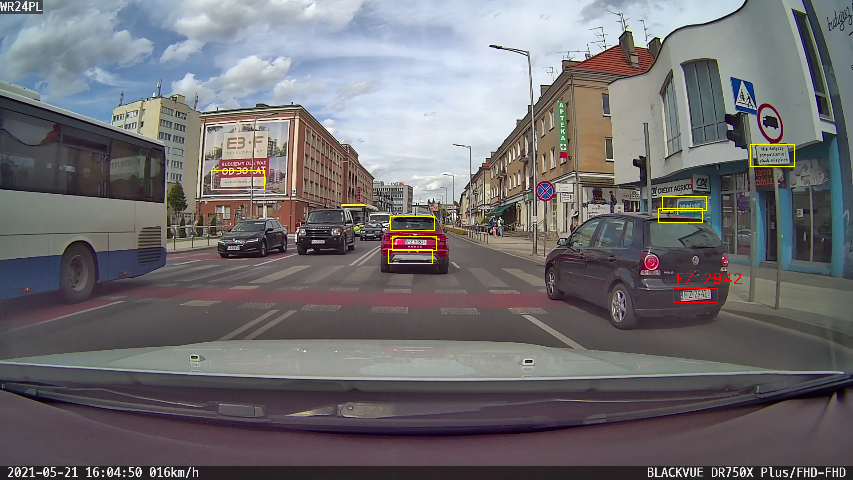
\includegraphics[scale=0.4]{Pictures/tablica_rozpoznana}
    \caption{Wyniki detekcji tablic rejestracyjnych dla progu $t=1.5$. Liczba cech $T=64$ (źródło: opracowanie własne).}
    \label{fig:tablica_rozpoznana}
\end{figure}
\FloatBarrier
Innym przykładem błędnej detekcji jest Rysunek~\ref{fig:autobus}.
Jako pozytyw oznaczono wyświetlacz autobusu, zawierający informację o numerze linii autobusowej.
\begin{figure}[!ht]
    \centering
    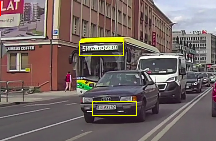
\includegraphics[scale=1]{Pictures/autobus}
    \caption{Wyświetlacz na autobusie wykryty jako tablica rejestracyjna dla progu $t=1.5$. Liczba cech $T=64$ (źródło: opracowanie własne).}
    \label{fig:autobus}
\end{figure}
\FloatBarrier
Kolejnym przykładem błędnej detekcji jest Rysunek~\ref{fig:bank}.
Jako pozytyw wykryto szyld banku.
Podobnie jak w przypadku wyświetlacza na autobusie, okno zawiera kontrastowy tekst.
\begin{figure}[!ht]
    \centering
    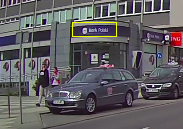
\includegraphics[scale=1]{Pictures/bank}
    \caption{Szyld reklamowy wykryty jako tablica rejestracyjna dla progu $t=1.5$. Liczba cech $T=64$ (źródło: opracowanie własne).}
    \label{fig:bank}
\end{figure}
\FloatBarrier
Z przedstawionymi błędami można walczyć za pomocą umiejętnego dobierania progu decyzyjnego $t$.
Dla progu $t=2.5$ powyższe okna nie zostają uznane za pozytywne.
Zwiększanie progu jednak objawia się również brakiem detekcji dla niektórych próbek pozytywnych.
Rysunek~\ref{fig:same_car} przedstawia problem braku detekcji tego samego samochodu pomiędzy klatkami.
Takie zachowanie wynika z nieprzekroczenia progu dla środkowego zdjęcia.
\begin{figure}[!ht]
    \centering
    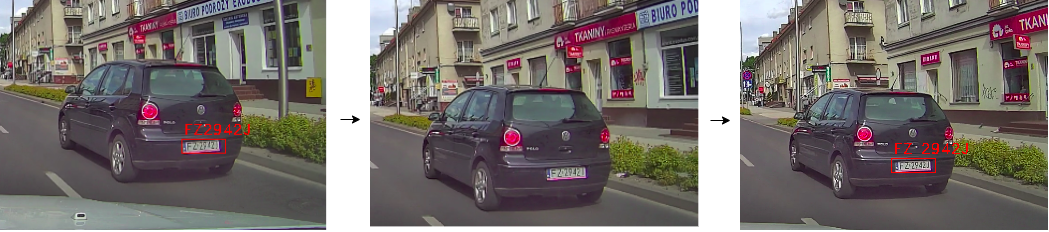
\includegraphics[scale=0.4]{Pictures/same_car}
    \caption{Brak detekcji tego samochodu pomiędzy klatkami dla progu $t=2.5$. Liczba cech $T=64$ (źródło: opracowanie własne).}
    \label{fig:same_car}
\end{figure}
\FloatBarrier
Warto również zaznaczyć fakt, że niektóre tablice są nieczytelne nawet dla ludzkiego oka.
Ludzki umysł niejako się domyśla, że z przodu lub z tyłu samochodu znajduje się tablica rejestracyjna, nawet jeżeli na zdjęciu bardziej przypomina biały prostokąt.
Opracowany klasyfikator nie ma takiej wiedzy.
Z tego powodu, określenie granicy, dla której próbki powinny być klasyfikowane jako pozytywne, nie jest trywialnym zadaniem.

Należy podkreślić, że procent poprawnie sklasyfikowanych próbek przez klasyfikator nie zawsze powinien być jedyną miarą jakości systemu.
Przykładowo, dla obrazu przedstawionego na Rysunku~\ref{fig:tablica_rozpoznana} procedura oknem przesuwnym, dla liczby cech równej 2205 oraz rozmiaru okna
45$\times$15px, generuje 39188 okien.
Jeżeli uznamy, że 20 okien zostało źle sklasyfikowanych, to poprawność klasyfikacji dalej jest bardzo wysoka i wynosi w tym przypadku $99.95\%$.


\section{Wyniki rozpoznawaniu znaków}
Jak wspomniano w poprzednim rozdziale, do rozpoznawania tekstu wykorzystano bibliotekę Tesseract.
Zgodnie z~\cite{sym12050715}, dokładność klasyfikacji biblioteki wynosi $70.2\%$.
W rzeczywistości, jakość działania systemu w głównej mierze zależy od metod segmentacji znaków.
Na Rysunku~\ref{fig:plates} zaprezentowano przykładowe wyniki segmentacji znaków z tablic rejestracyjnych.
\begin{figure}[!ht]
    \centering
    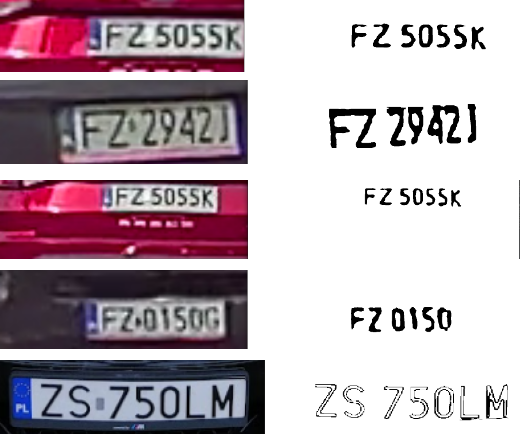
\includegraphics[scale=0.4]{Pictures/plates}
    \caption{Przykładowe wyniki segmentacji znaków z tablic rejestracyjnych (źródło: opracowanie własne).}
    \label{fig:plates}
\end{figure}
\FloatBarrier
Można przyjąć założenie, że im tablica jest większa, tym algorytm uzyskuje lepsze wyniki.
Wynika to przede wszystkim z mniejszych zakłóceń w obrazie i lepiej widocznych przerwach pomiędzy znakami.

Na jakość segmentacji i następnie odczytu znaków wpływ ma również rotacja tablicy rejestracyjnej.
Dodatkowo, w zależności od kąta, pod którym zrobiono zdjęcie, kontury znaków potrafią się łączyć ze sobą lub z ramką tablicy.
Ten fakt zdecydowanie nie ułatwia późniejszej segmentacji.
%TODO - przedstawienie rozpoznawania na podstawie zdjęć
%\\przykłady:
%\\mylony znak ``('' z ``J''
%\\mylone S z 5


\section{Porównanie wydajności czasowej}
Dla systemów automatycznego rozpoznawania tablic rejestracyjnych wydajność jest jedną z kluczowych kwestii.
Aby dane mogły być odpowiednio przetwarzane, system powinien na bieżąco procesować zdjęcia.
Wydajność jest uzależniona od poniższych czynników:
\begin{itemize}
    \item rozmiar okna przesuwnego,
    \item liczna skal dla okna przesuwnego,
    \item liczba pozytywnych okien wysłanych do modułu rozpoznawania znaków,
    \item liczba cech klasyfikatora.
\end{itemize}

\begin{table}[h]
    \centering
    \caption{Wydajność czasowa systemu.}
    \label{tab:performance}
    \begin{tabular}{c c c c c c}
        \toprule
        \textbf{\thead{Liczba \\cech}} & \textbf{\thead{Liczba  \\słabych \\klasyfikatorów}} & \textbf{\thead{Liczba \\koszyków}} & \textbf{\thead{Dokładność \\klasyfikatora}} & \textbf{\thead{Dokładność \\klasyfikatora dla \\próbek pozytywnych}} & \textbf{\thead{Dokładność \\klasyfikatora dla \\próbek negatywnych}} \\
        \midrule
        2205 & 32 & 8 & ???\%  & ???\%  & ???\%  \\
        2205 & 64 & 8 & 99,8\%  & 82,2\%  & 99,9\%  \\
        2205 & 128 & 8 & ???\%  & ???\%  & ???\%  \\
        2205 & 256 & 8 & ???\%  & ???\%  & ???\%  \\
        \bottomrule
    \end{tabular}
\end{table}


\section{Propozycje udoskonalenia}
TODO